\chapter{Soluci�n}\label{solucion}
\lhead{Cap�tulo \ref{solucion}}
\rhead{Descripci�n detallada de la soluci�n}
%*******************************************************************************
%%%%%%%\section{Identificaci�n y gesti�n de riesgos}\label{idGestRiesgos}
%*
%*
%*
%*
%*
%*

	%%%%%%%%\subsection{Identificaci�n de riesgos}\label{identificacionRiesgos}
	
	\begin{figure}[htbp]
		\centering
			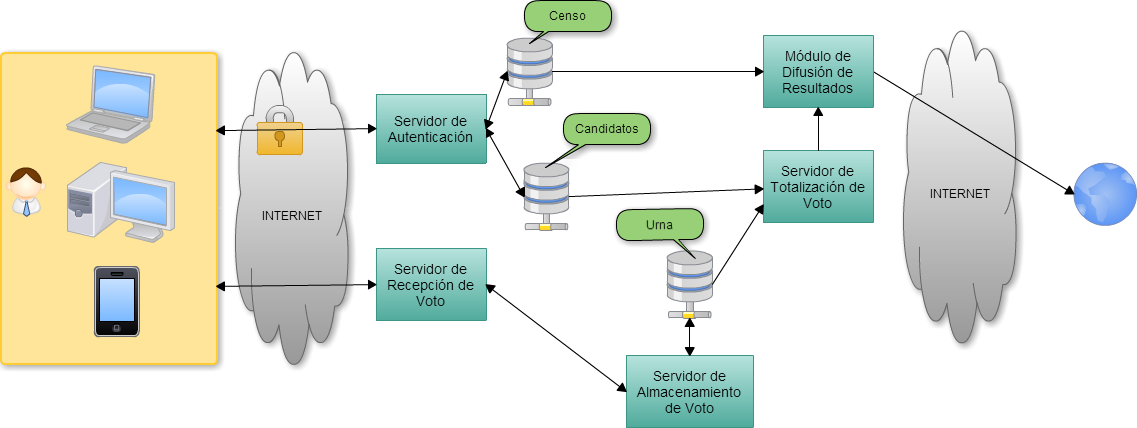
\includegraphics[width=1\textwidth]{imgs/sistema.png}
		\caption{Diagrama de flujo del Sistema}
		\label{fig:sistema}
	\end{figure}
	
	\begin{figure}[htbp]
		\centering
			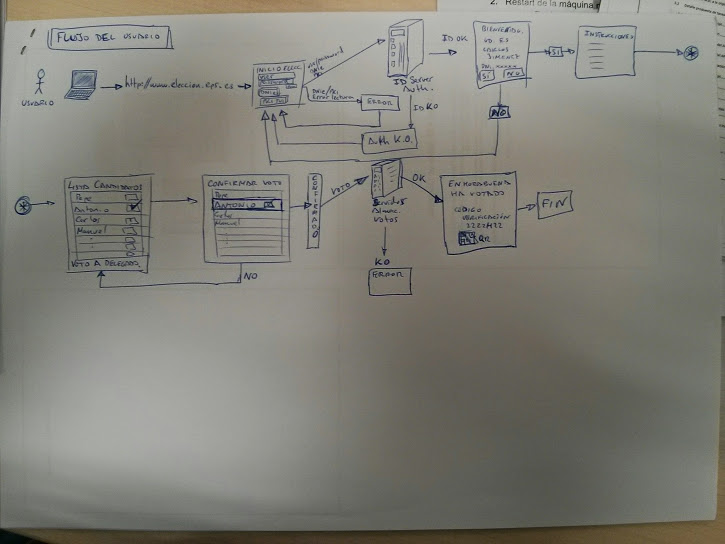
\includegraphics[width=0.60\textwidth]{imgs/flujoUsuario.jpg}
		\caption{Esquema del flujo que sigue el votante}
		\label{fig:flujoUsuario}
	\end{figure}
	\begin{figure}[htbp]
		\centering
			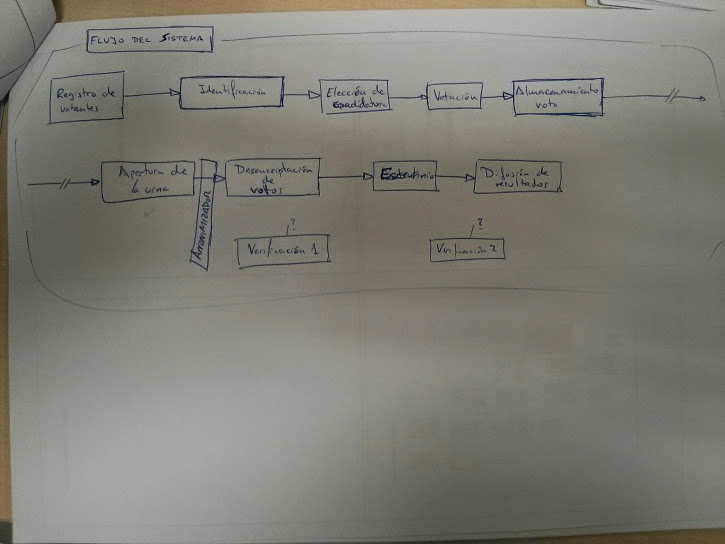
\includegraphics[width=0.60\textwidth]{imgs/flujoSistema.jpg}
		\caption{Esquema del flujo del Sistema}
		\label{fig:flujoSistema}
	\end{figure}
	
	
	

	\section{Roles}
		Considerando el flujo del votante en el sistema, identificamos 4 roles en el sistema que deben ser tenidos en cuenta de cara a las funcionalidades, privilegios y responsabilidades que tienen que encontrar en el uso del mismo.
		\begin{itemize}
			\item Votante
			\item Administrador
				El administrador es el rol encargado de gesti�n de las fases electorales.\\
				Tiene responsabilidad y potestad de:
					\begin{itemize}
						\item Iniciar el proceso electoral.
						\item Iniciar el proceso de votaci�n.
						\item Terminar el proceso de votaci�n.
						\item Apertura de la urna
						\item Apertura de los canales de difusi�n de resultados.
					\end{itemize}
				Los usuarios con este rol no puede votar. El administrador de la elecci�n no forma parte del censo de votantes acreditados para votar en las elecciones, por lo que no puede tener acceso al m�dulo de votaci�n.
			\item Miembro de la Junta Electoral ***************** CAMBIAR EL NOMBRE ***********************
				Una vez el administrador de la elecci�n d� por finalizado el proceso electoral, se requerir� que varios miembros de la Junta Electoral proporcionen unas claves personales que, juntando varias de ellas, servir�n como llave l�gica para la apertura de la urna que contiene los votos.\\
				Los usuarios con este rol no puede votar. El miembro de la Junta Electoral no forma parte del censo de votantes acreditados para votar en las elecciones, por lo que no puede tener acceso al m�dulo de votaci�n.
			\item Auditor
				El auditor debe tener acceso a una serie de funcionalidades del sistema. Su funci�n es velar porque el desarrollo del proceso electoral se realiza sin ning�n tipo de fallo o de interferencia por parte de alg�n atacante.\\
				Los usuarios con este rol no puede votar. El auditor no forma parte del censo de votantes acreditados para votar en las elecciones, por lo que no puede tener acceso al m�dulo de votaci�n.\\
				Su misi�n es de control, por lo que ninguna acci�n que realice en el sistema puede afectar al desarrollo de la elecci�n.
		\end{itemize}